\documentclass{article}
\usepackage{tikz}
\begin{document}
\begin{center}
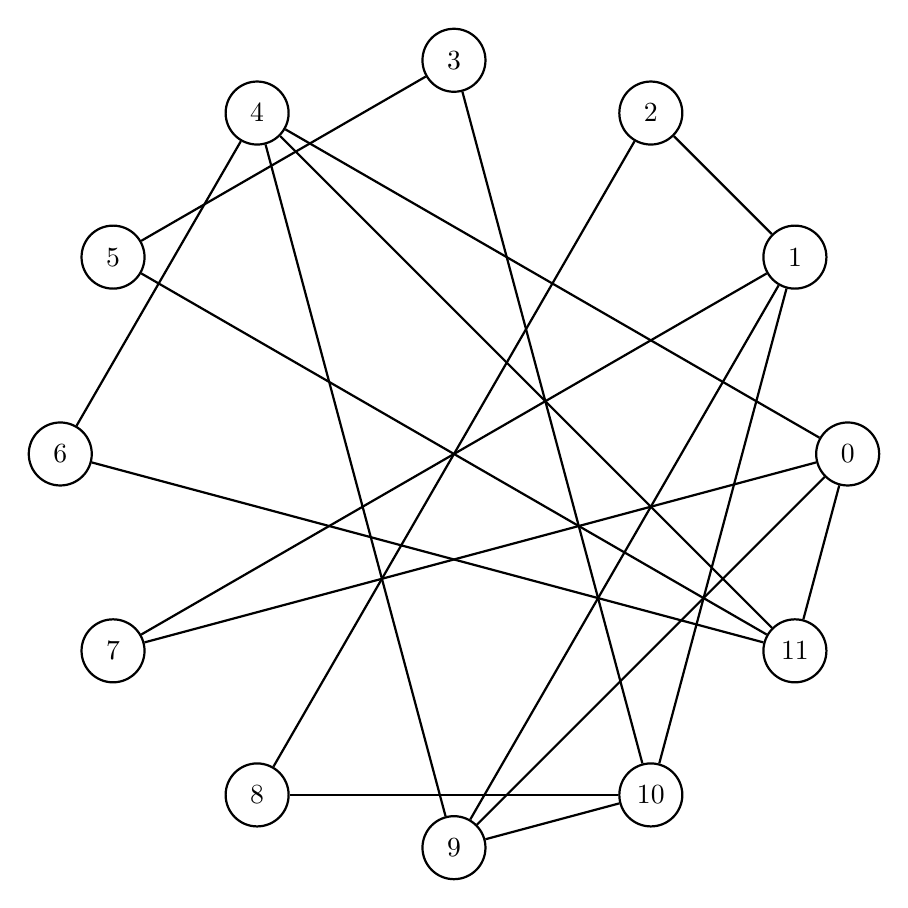
\begin{tikzpicture}[auto, node distance=3cm, thick]
\tikzstyle{every node}=[circle,draw,minimum size=8mm,inner sep=1pt]

\node (0) at (5.00,0.00) {0};
\node (1) at (4.33,2.50) {1};
\node (2) at (2.50,4.33) {2};
\node (3) at (0.00,5.00) {3};
\node (4) at (-2.50,4.33) {4};
\node (5) at (-4.33,2.50) {5};
\node (6) at (-5.00,0.00) {6};
\node (7) at (-4.33,-2.50) {7};
\node (8) at (-2.50,-4.33) {8};
\node (9) at (-0.00,-5.00) {9};
\node (10) at (2.50,-4.33) {10};
\node (11) at (4.33,-2.50) {11};

\draw (9) -- (10);
\draw (0) -- (7);
\draw (1) -- (2);
\draw (0) -- (4);
\draw (5) -- (11);
\draw (6) -- (11);
\draw (4) -- (9);
\draw (4) -- (6);
\draw (0) -- (9);
\draw (3) -- (10);
\draw (8) -- (10);
\draw (1) -- (7);
\draw (3) -- (5);
\draw (1) -- (10);
\draw (4) -- (11);
\draw (1) -- (9);
\draw (0) -- (11);
\draw (2) -- (8);
\end{tikzpicture}
\end{center}
\end{document}
